% ---------------------------- %
% Assignment Report Template
% 
% Heidi Christensen, 2020
% --------------------------   %


\documentclass[11pt,oneside]{article}
\usepackage[utf8]{inputenc}
\usepackage{graphicx}
\usepackage{algorithm}% http://ctan.org/pkg/algorithm
\usepackage{algpseudocode}% http://ctan.org/pkg/algorithmicx
\usepackage{multirow}

\title{Experimental report for the 2021 COM1005 Assignment: The Rambler's Problem\footnote{https://github.com/aronjyl/COM1005}}
\author{YiLong Jia}
\date{}


\begin{document}
\maketitle
In this report, we firstly describe the implementation of Branch and Bound~(BB) and A* search. Then, we will evaluate the efficiency of these two approaches in different maps and evaluation functions based on the presented results.

% 
% TODO: 
% 1. simple algorithm description; and 4 eval functions
% 2. avg and std results from 1K on diablo and tmc (table)
% 3. all results from 50 on diablo and tmc (bar char)
% 4. results include 4 different evaluation 

\section{Description of Branch-and-Bound and A* implementation}
My BB search will explore the node with the lowest accumulated cost, it uses an \textbf{open list} to keep track of nodes that yet to explore, and it is sorted based on the accumulated cost. There is also a \textbf{closed list} that keeps track of nodes are already visited. Then, BB search will continue to iterate all nodes in the given procedure till it reaches the goal.% as displayed in Algorithm~\ref{bb_algo}.

% \begin{algorithm}
%   \caption{Branch and Bound}\label{bb_algo}
%   \begin{algorithmic}[1]
%     \Procedure{Branch and Bound Search}{$a, b$} 
%       \State $r\gets a\bmod b$
%       \While{open list is not empty} 
%         \State $a\gets b$
%         \State $b\gets r$
%         \State $r\gets a\bmod b$
%         \For{$i = 1$ to $N$}
%           \State select the lowest accumulated cost node
%         \EndFor        
%       \EndWhile
%       \State \textbf{return} $b$ 
%     \EndProcedure
%   \end{algorithmic}
% \end{algorithm}

In addition, A* search algorithm builds on a heuristic function that is based on the sum of $g(n)$, which is known cost of getting from start to the current node~(n), and $f(n)$, which is the estimated of remaining cost from the current node~(n) to the goal. % as in Algorithm~\ref{astar_algo}.

Therefore, in RamblersState.java, the RamblerSearcher will find all valid successors around the current node, that will be iterating 4 different directions $\{\{1,0\},\{0,1\},\{-1,0\},\{0,-1\}\}$, and we will ignore all invalid nodes that meet one of 4 conditions that checks whether this node has exceed the boundary of this map.

 \begin{figure}[H]
\centering
  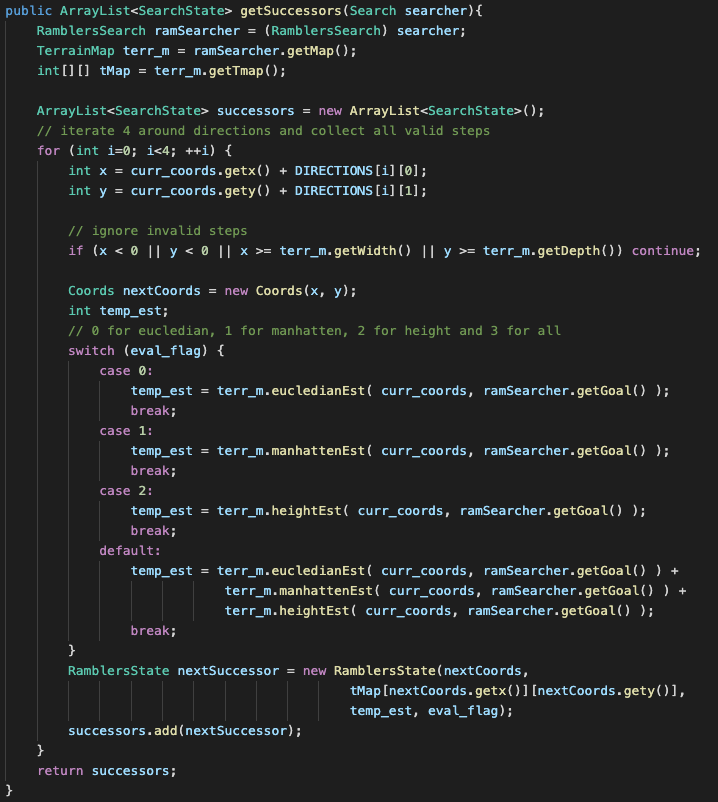
\includegraphics[scale=0.45]{getSuccessors.png}
  \caption{getSuccessors() for RamblersState}
  \label{fig:getsuccessor}
 \end{figure}
Moreover, we have evaluated 4 different distances for the A* search in TerrainMap.java as displayed in Fig~\ref{fig:eval_fnc}, so RamblersState will use an instance of TerrainMap to evaluate the cost and decide the next successors, as displayed in the Fig~\ref{fig:getsuccessor}.

\begin{figure}[H]
\centering
  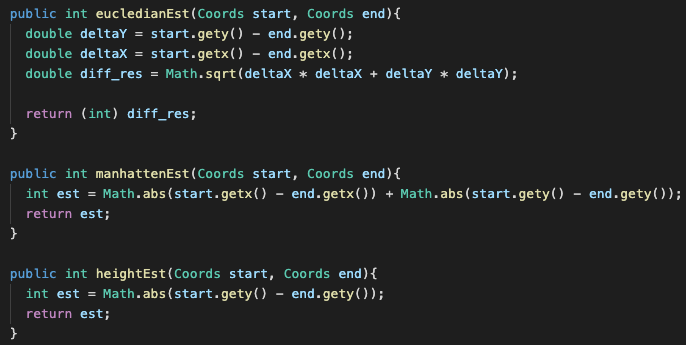
\includegraphics[scale=0.45]{eval_fnc.png}
  \caption{Evaluation functions in TerrainMap}
  \label{fig:eval_fnc}
 \end{figure} 
 

\begin{itemize}
  \item Manhattan distance, $d_m(x, y) = \sum_{i=1}^n |x_i - y_i|$
  \item Euclidean distance, $d_e(x, y) = \sum_{i=1}^n \sqrt{x^2_i - y^2_i}$
  \item Height distance, $d_h(y_i, y_j) = |y_i - y_j |$
  \item Combinations of all above three, $D = d_m + d_e + d_h$
\end{itemize}
% \begin{algorithm}
%   \caption{A* Star Search}\label{astar_algo}
%   \begin{algorithmic}[1]
%     \Procedure{A* Star}{$a, b$} 
%       \State $r\gets a\bmod b$
%       \While{open list is not empty} 
%         \State $a\gets b$
%         \State $b\gets r$
%         \State $r\gets a\bmod b$
%         \For{$i = 1$ to $N$}
%           \State $h(n) = g(n) + f(n)$
%         \EndFor        
%       \EndWhile
%       \State \textbf{return} $b$ 
%     \EndProcedure
%   \end{algorithmic}
% \end{algorithm}

% \begin{table}[ht]
%     \centering
%     \begin{tabular}{|c|c|}
%         System      & Measurement [\%] \\ \hline
%         Basic       & 40\% \\
%         Improved v1 & 42\% \\
%         Improved v2 & 43\% \\
%     \end{tabular}
%     \caption{Example table}
%     \label{tab:my_label}
% \end{table}

\section{Assessing efficiency}
We evaluated the A* search in $100$ random locations in two different maps by 4 different costs~(Euclidean, Manhattan, Height and the combined all), and the result is displayed in Fig~\ref{fig:eval_as_costs}, the y-axis is the efficiency that means A* search is more efficient than B\&B in general and A* search is affected by the choice of evaluation distance, and the combined all costs together has the most advantage in the efficiency performance. 

 \begin{figure}[H]
\centering
  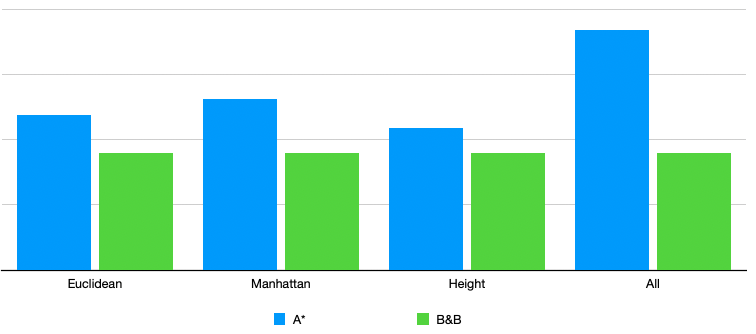
\includegraphics[scale=0.5]{eval_as_cost.png}
  \caption{The average performance evaluation on A* at 4 different costs}
  \label{fig:eval_as_costs}
 \end{figure}

 
\subsection{Assessing the efficiency of my branch-and-bound and A* search algorithm}
We generated 1000 random start and end locations in the target map, and evaluate BB search algorithm. The average efficiency result for 1000 times is $0.13$ and the standard deviation is $0.12$.

\begin{table}[H]
\begin{tabular}{|c|c|c|c|c|}
\hline
\multirow{2}{*}{} & \multicolumn{2}{c|}{Branch \& Bound} & \multicolumn{2}{c|}{A* Star} \\ \cline{2-5} 
 & avg. efficiency & std & avg. efficiency & std \\ \hline
tmc.pgm & 0.117 & 0.108 & 0.124 & 0.084 \\ \hline
diablo.pgm & 0.125 & 0.106 & 0.162 & 0.077 \\ \hline
\end{tabular}
\caption{Evaluation B\&B and A* star in 1000 random locations}
\label{tab:eval_table}
\end{table}

\section{Conclusions}
Based on our evaluation on two maps~(tmc.pgm and diablo.pgm), we can see A* star search is better than BB in terms of efficiency performance, and its performance is affected by the choice of evaluation function.

\end{document}
